\newpage\section{Continuidade e Descontinuidade}Em uma situação onde temos uma superfície $S$ onde há uma densidade de carga $\sigma$  e um campo elétrico $\Vec{E}$ que está perpendicular a superfície $S$. Nesse caso fica a questão de saber se o campo elétrico $\Vec{E}$ será o mesmo ao atravessar a superfície $S$. 
Primeiramente podemos utilizar a lei de Gauss, onde 
\begin{equation}
    \oint \Vec{E}_{tot} \cdot d\mathbf{a} = \frac{Q_{enc}}{\epsilon_{0}} = \frac{\sigma A}{\epsilon_{0}},
\end{equation}
onde $A$ é a área da superfície gaussiana. Como $E_{tot}$ é o campo elétrico total, então 

\begin{equation}
    \left(\oint \Vec{E}_{acima} da\right) \cdot \hat{n} +\left(\oint \Vec{E}_{abaixo} da\right) \cdot\hat{n} = \frac{\sigma A}{\epsilon_{0}}
\end{equation}
como o vetor normal $\hat{n}$ é um vetor que sai da superfície, então o vetor normal do campo elétrico abaixo será o oposto do campo acima - já que estão em direção oposta - com isso
\begin{equation*}
    \left(\oint\Vec{E}_{acima} \cdot da -\oint \Vec{E}_{abaixo} \cdot da\right) \cdot \hat{n} = \frac{\sigma A}{\epsilon_{0}},
\end{equation*}
resultando em 

\begin{equation}
    \Vec{E}_{acima} - \Vec{E}_{abaixo} = \frac{\sigma}{\epsilon_{0}}.
\end{equation}
\myequations{Equação da descontinuidade do campo elétrico}
Com esse resultado vemos que quando o campo for perpendicular ao passar pela superfície S, o campo elétrico \(\Vec{E}_{acima}\) será diferente do campo elétrico abaixo \(\Vec{E}_{abaixo}\), isto é, ele será  \textbf{descontínuo} com um fator $\sigma/\epsilon_0$. 


   % 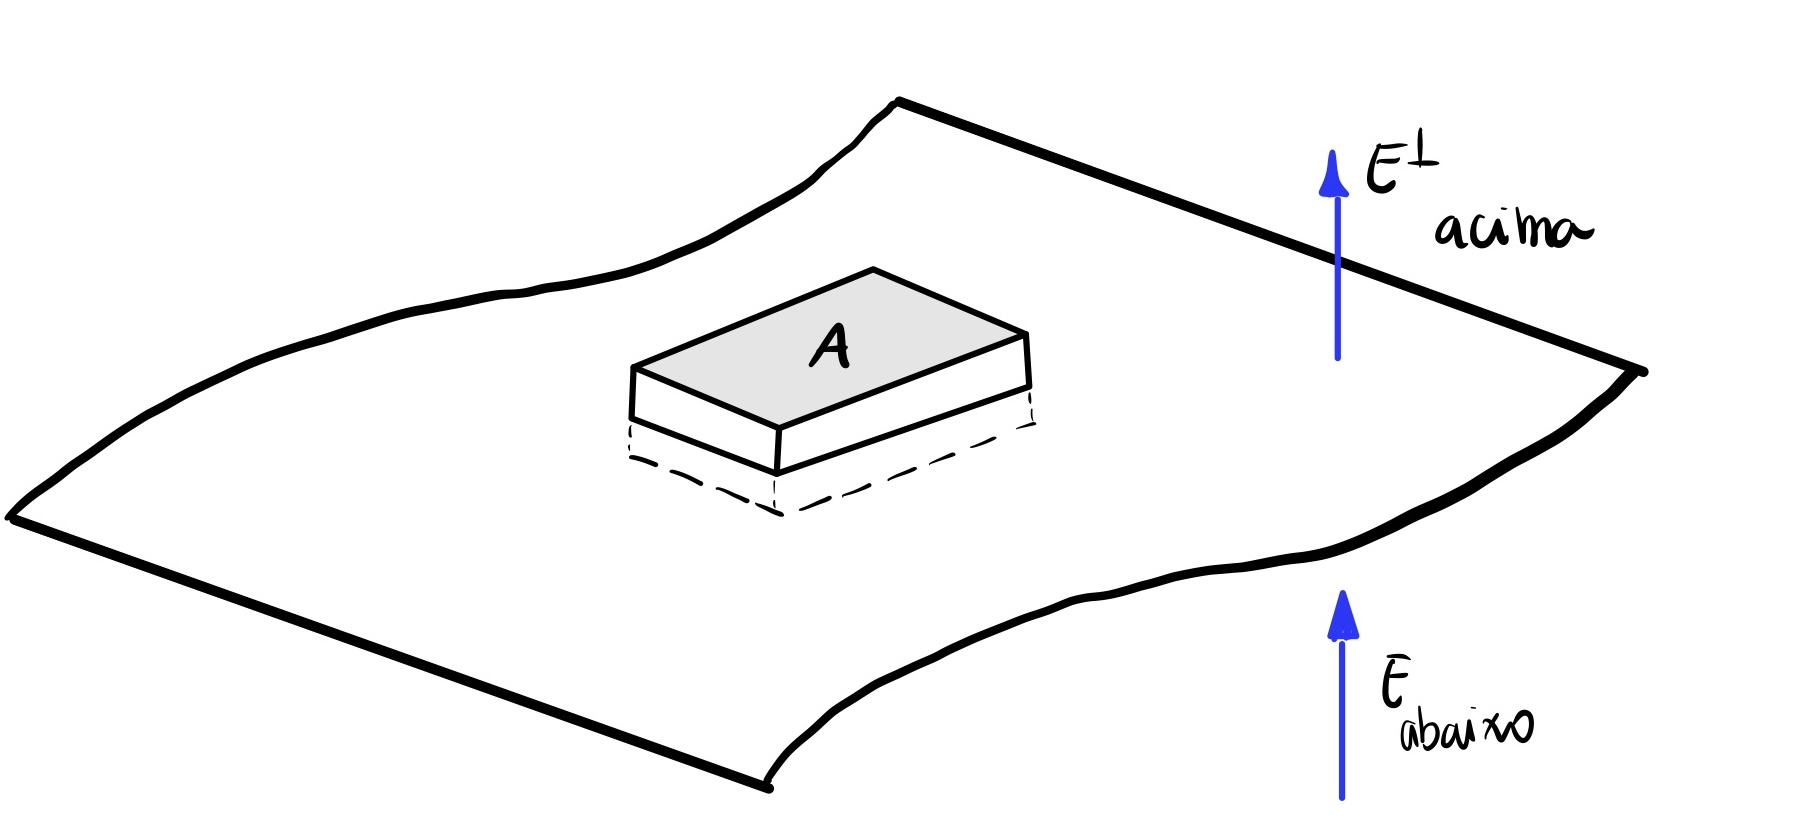
\includegraphics[width=0.5\linewidth]{IMG_3012.jpeg}
    

Agora quando o campo elétrico está tangente ao campo elétrico não haverá \textbf{descontinuidade}, porque as linhas de campo serão ortogonais, então o produto escalar entre eles dará que o ângulo do cosseno será igual a zero.  Com isso teremos que

\begin{equation}\label{seila}
    \Vec{E}_{acima} - \Vec{E}_{abaixo} = \frac{\sigma}{\epsilon_{0}} \hat{\vec{n}}
\end{equation}
\(\hat{n}\) será igual a $0$ (zero), consequentemente 


\[\Vec{E}_{acima} - \Vec{E}_{abaixo} = \frac{\sigma}{\epsilon_{0}} \cdot 0 \xrightarrow{}\Vec{E}_{acima} = \Vec{E}_{abaixo}\]




%\begin{figure}[h]
    %\centering
    %\caption{Campo elétrico tangente a superfície}
    %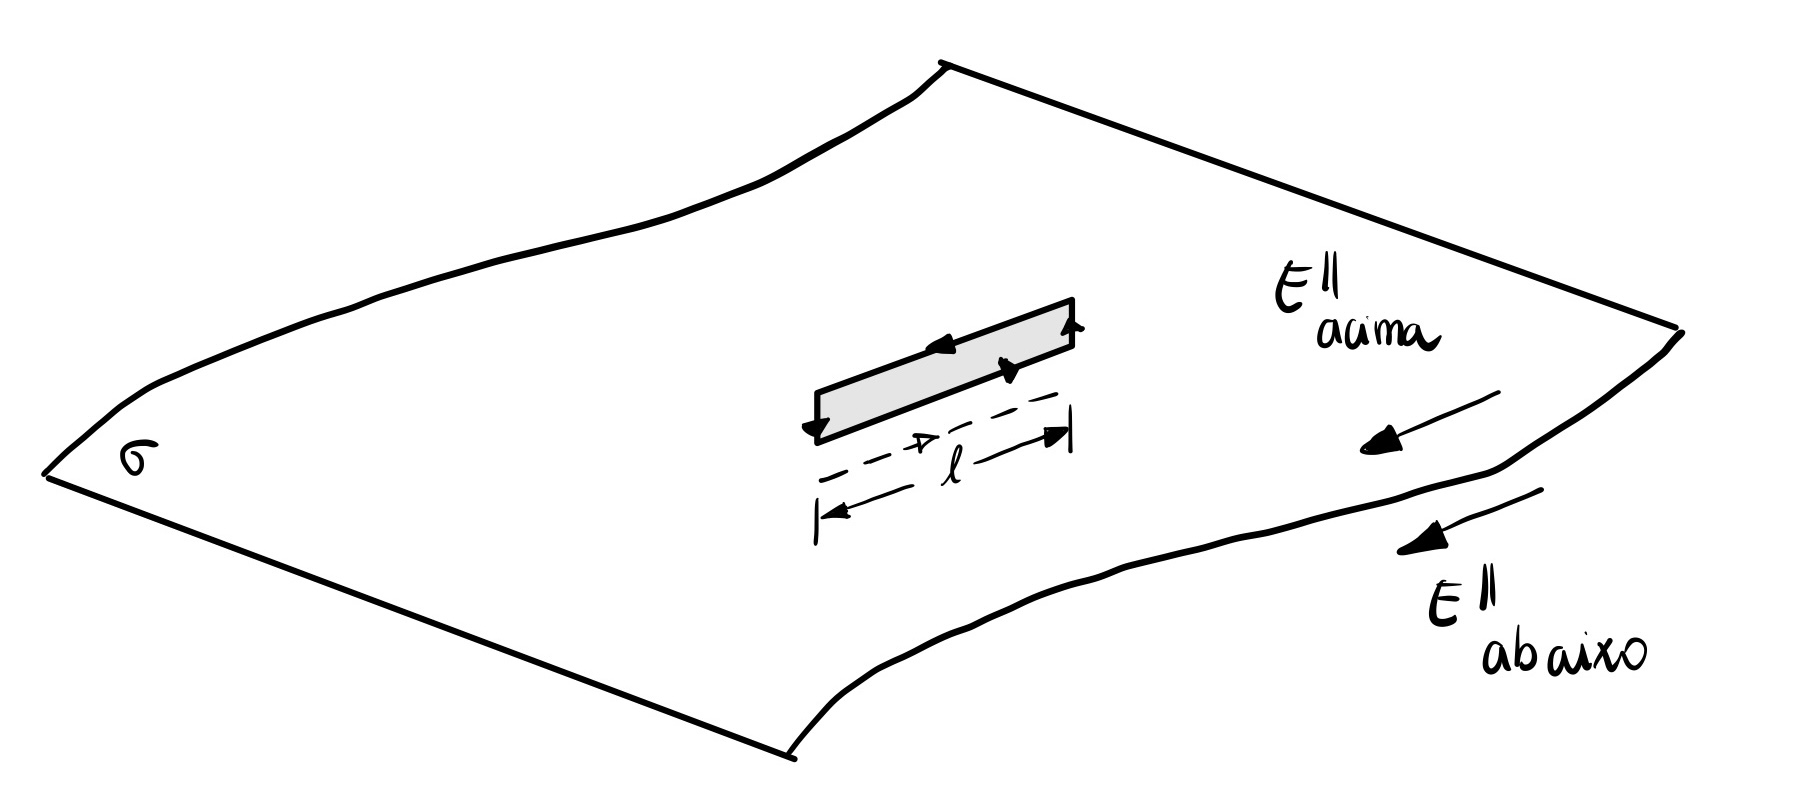
\includegraphics[width=0.5\linewidth]{IMG_3013.jpeg}
    
 %   \label{fig:enter-label}
%\end{figure}


O \textbf{potencial} entre dois pontos é dado por

\[V(b)-V(a) = - \int_{O}^{b} E\cdot d\textbf{l} +\int_{O}^{a} E\cdot d\textbf{l} \]
\[V(b)-V(a) = - \int_{a}^{b} E\cdot d\textbf{l}.\]
Quando há uma superfície entre os pontos temos


\[V_{acima} - V_{abaixo} = - \int_{a}^{b} E \cdot d\textbf{l},\]
conforme a distância entre os pontos $a$ e $b$ vai diminuindo, ficando próxima a espessura da superfície, a integral tende a zero, logo 


\[V_{acima} = V_{abaixo},\]
isto é, não há descontinuidade. Mas quando aplicamos o divergente na equação \ref{seila} (já que \(E = -\nabla V\)) temos que
\[\nabla V_{acima}-\nabla V_{abaixo} = -\frac{\sigma}{\epsilon_{0}} \hat{\textbf{n}}\]
implicando que por mais que o potencial não tenha descontinuidade o gradiente dele terá. Como o campo elétrico $E$ é igual a menos o gradiente do potencial então poderia - eu suponho - que dá para afirmar que caso o campo seja descontinuo o negativo do gradiente do potencial também será descontinuo, sem fazer conta alguma. 